%%%%%%%%%%%%%%%%%%%%%%%%%%%%%%%%%%%%%%%%%%%%%%%%%%%%%%%%%%%%%%%%%%%%%%%%%%%
%
% Plantilla para un artículo en LaTeX en doble columna.
%
%%%%%%%%%%%%%%%%%%%%%%%%%%%%%%%%%%%%%%%%%%%%%%%%%%%%%%%%%%%%%%%%%%%%%%%%%%
% !TeX spellcheck = es_ANY
%\documentclass[11pt,twocolumn]{article} %doble columna
%\documentclass[11pt]{article}

\documentclass[journal, onecolumn]{IEEEtran}
\IEEEoverridecommandlockouts
% The preceding line is only needed to identify funding in the first footnote. If that is unneeded, please comment it out.

\usepackage{url}
\usepackage[utf8]{inputenc}
\usepackage[english]{babel}
\usepackage{fullpage}
\usepackage{graphicx}
\usepackage{array}

% Paquetes de la AMS:
\usepackage{amsmath, amsthm, amsfonts, amssymb}

% Atajos.
% Se pueden definir comandos nuevos para acortar cosas que se usan
% frecuentemente. Como ejemplo, aquí se definen la R y la Z dobles que
% suelen representar a los conjuntos de números reales y enteros.
%--------------------------------------------------------------------------

\def\RR{\mathbb{R}}
\def\ZZ{\mathbb{Z}}

% De la misma forma se pueden definir comandos con argumentos. Por
% ejemplo, aquí definimos un comando para escribir el valor absoluto
% de algo más fácilmente.
%--------------------------------------------------------------------------
\newcommand{\abs}[1]{\left\vert#1\right\vert}


%--------------------------------------------------------------------------
\title{Identification of rice genes which respond to saline stress from co-expression networks analysis}
\author{Camila Riccio Rengifo\\
  \small Pontificia Universidad Javeriana Cali\\
}

\begin{document}

\maketitle


\section*{Introduction}
Abiotic stresses are the key factors which negatively influence plant development and productivity. They are the main cause of extensive agricultural production losses worldwide. One of the most devastating abiotic stresses, causing reduction in the cultivable land, crop quality and productivity is soil salinity. It has been estimated that 20\% of total cultivated and 33\% of irrigated agricultural lands worldwide are already affected by high salinity. Due to the human activities and natural causes, salinized areas are gradually increasing every year and are expected to reach 50\% by the end of year 2050~\cite{shrivastava2015soil}. Salinity effects are the result of elaborated interactions among morphological, physiological, and biochemical processes. Those processes are regulated by multiple genes and determine the salt tolerance or susceptibility of the crop~\cite{reddy2017salt}. Thus, identifying this group of stress responsive genes may lead to crop improvement in salt tolerance, which is known as a complex quantitative trait. Find this target genes is a complex task, because the function of many genes are still not understood and many novel non-coding genes have been discovered. Particularly rice (\textit{Oryza sativa}), the major food source around the world, is highly sensitive to salt stress~\cite{chang2019morphological}. Therefore, identification of target genes in rice may allow biologist use them as a genetic resource to develop new cultivars with resistance to salinity.\\

We propose a methodology to identify stress responsive genes to salt conditions in rice. The methodology is based on Weighted Gene Co-expression Network Analysis (WGCNA). This is considered an effective and accurate bioinformatic method, using co-expression networks, that has been widely applied in identifying target genes for disease and cancer fields~\cite{tian2018identifying}. We follow the WGCNA workflow but with a new approach in the module detection step. Our modules are detected using the Hierarchical Link Clustering (HLC) technique~\cite{ahn2010link} that allows the recognition of overlapping communities, which may have more biological meaning given the overlapping regulatory domains of systems that generate co-expression~\cite{gaiteri2014beyond}. We conduct a systematic study with a large set of rice data using the proposed methodology. RNA-seq data was accessed through GEO database~\cite{GEOAcces90:online} (Accession number GSE98455), corresponding to $57845$ gene expression profiles of shoot tissues measured for both control and salt condition in $92$ accessions of the Rice Diversity Panel 1. As the analysis result, 6 modules are detected as relevant in the response to salt stress in rice: 3 modules of 3 genes each one associated with shoot K content, 2 modules of 3 genes associated with  shoot biomass, and 1 module of 4 genes associated with root biomass. These genes may act as potential targets for the improvement of salinity tolerance in rice cultivars. From those 19 genes, all but 3 genes (associated with $K$ content), were also identified as deferentially expressed ($|LFC| > 2$) for at least one of the 92 accessions, suggesting that those genes are strong candidates as stress responsive genes. Only 2 of the 16 diferentially expressed genes, both from the module related with shoot biomass, are named and have an associated protein product: Spermidine hydroxycinnamoyltransferase 2 (SHT2) and Lipoxygenase. In other words, further studies are needed to elucidate the detailed biological function of the remaining 14 genes that have not been named so far,  which may have a potential relevance in stress responsive mechanisms to salt conditions in rice.\\

With the development of high-throughput technologies, including microarrays and RNA sequencing (RNA-seq), genome-wide gene expression can be studied under different environmental stimuli (e.g. salt stress). Our methodology uses this kind of transcriptomic data measured for two different conditions (control and stress). After a process of normalization and filtering of the raw data, a differential expression profile of the genes is built calculating the log fold change (LFC) from control to stress condition. The LFC matrix will be the input for the co-expression network construction trough the WGCNA method. A similarity matrix is calculated using the absolute value of Pearson's correlation coefficient between pairs of genes. Then, the similarity matrix is forced to be a scale-free network, finding a beta exponent such that by raising each entry of the matrix to that value, the probability distribution follows a power law. Next, unlike WGCNA, the scale-free network is used to detect overlapping rather than non-overlapping communities, using the HLC technique. We also implement a LASSO regression~\cite{tibshirani1996regression} to select the most significant modules associated with rice phenotypical responses to salt stress. Finally, for the genes found, we look for previous evidence of important biological implications in tolerance to salt stress. That is, the genes deferentially expressed within the selected modules are enriched with gene ontology annotations from QuikGO database~\cite{binns2009quickgo} and their interaction networks reported in STRING database~\cite{szklarczyk2016string} are reviewed.\\

The proposed methodology is modular, since other module detection and selection techniques could be used, instead HLC and LASSO respectively. The advantage of using HLC as clustering method is its ability to detect overlapping modules, since biological components are involved in multiple functions and therefore biological communities tend to be highly overlapping ( ). On the other hand, LASSO is a regularized regression technique widely used in variable selection, thanks to its ability to obtain zero regression coefficients for the less relevant variables~\cite{desboulets2018review}. Additionally, LASSO is especially useful in problems where the number of variables is much larger than the number of samples, which is our case having more than 5000 modules (variables) and 92 accession (samples). The combinations of these techniques would allow finding target genes for future biological studies that evaluate their potential as genes that respond to salt stress in rice. Furthermore, this study can be extended to other stresses and even to other crops.\\


\section{Methodology}
\subsection{Data pre-processing} 
The RNA-seq data cannot be directly interpreted, therefore a normalization process has to be done to deal with the various biases that affect quantification results. The normalization technique used was DESeq2 \cite{love2014moderated}. From the normalized data, the two biological repetitions of each accession were averaged and genes exhibiting low variance (the ratio of upper quantile to lower quantile smaller than 1.5) or low expression (more than 80\% samples with values smaller than 10) were removed. At this point, control and salinity stress treatment data are separated into two matrices $C=[c_{ij}]_{n \times p}$ and $T=[t_{ij}]_{n \times p}$, respectively, where $c_{ij}$ and $t_{ij}$ represent normalized expression level of the gene $i$ in the accession $j$.\\

Changes in gene expression between control and stress conditions, are measured in terms of log ratios. Matrix $L=[e_{ij}]_{n \times p}$, known as the Log Fold Change matrix, is computed by setting $\ell_{ij}=\log_2 (t_{ij}/c_{ij})$.\\

Genes with the ratio of upper quantile to lower quantile larger than $0.25$ were kept. This procedure aims to remove genes with low variance in the differential expression patterns. The final network contains $8928$ genes of the initial $57845$.

\subsection{Network construction}
The Log Fold Change matrix is used to construct the weighted co-expression network using the absolute value of the Pearson correlation as the similarity measure between genes. The matrix $S=[s_{ij}]_{n\times n}$ measures the level of concordance between gene expression profiles across experiments and is transformed into an adjacency matrix $A=[a_{ij}]_{n\times n}$ where $a_{ij} = (s_{ij})^\beta $ encodes the connection strength between each pair of genes. In other words, the elements of the adjacency matrix are the similarity values up to the power $\beta > 1$ so the degree distribution will fit a scale-free network. This kind of networks contain many nodes with very few connections and a small number of hubs with high connections. \\

In a strict scale-free network the logarithm of $P(k)$ (the probability of a node to have degree $k$) is approximately inversely proportional to the logarithm of $k$ (the degree of a node). So the parameter $\beta$ is chosen as the smallest value of $\beta$ such that the $R^2$ of the linear regression between $log_{10}(p(k))$ and $log_{10}(k)$ is close to $1$ (e.g. $R^2 > 0.85$). Figure~\ref{fig:beta} shows the degree distribution of the similarity matrix (left) and the degree distribution of the adjacency matrix (right) which is the degree distribution of a scale-free forced network with $R^2 = 0.8$ corresponding to $\beta = 3$.

%scale-free beta 1 y 3
\begin{figure}[h]
  \centering
    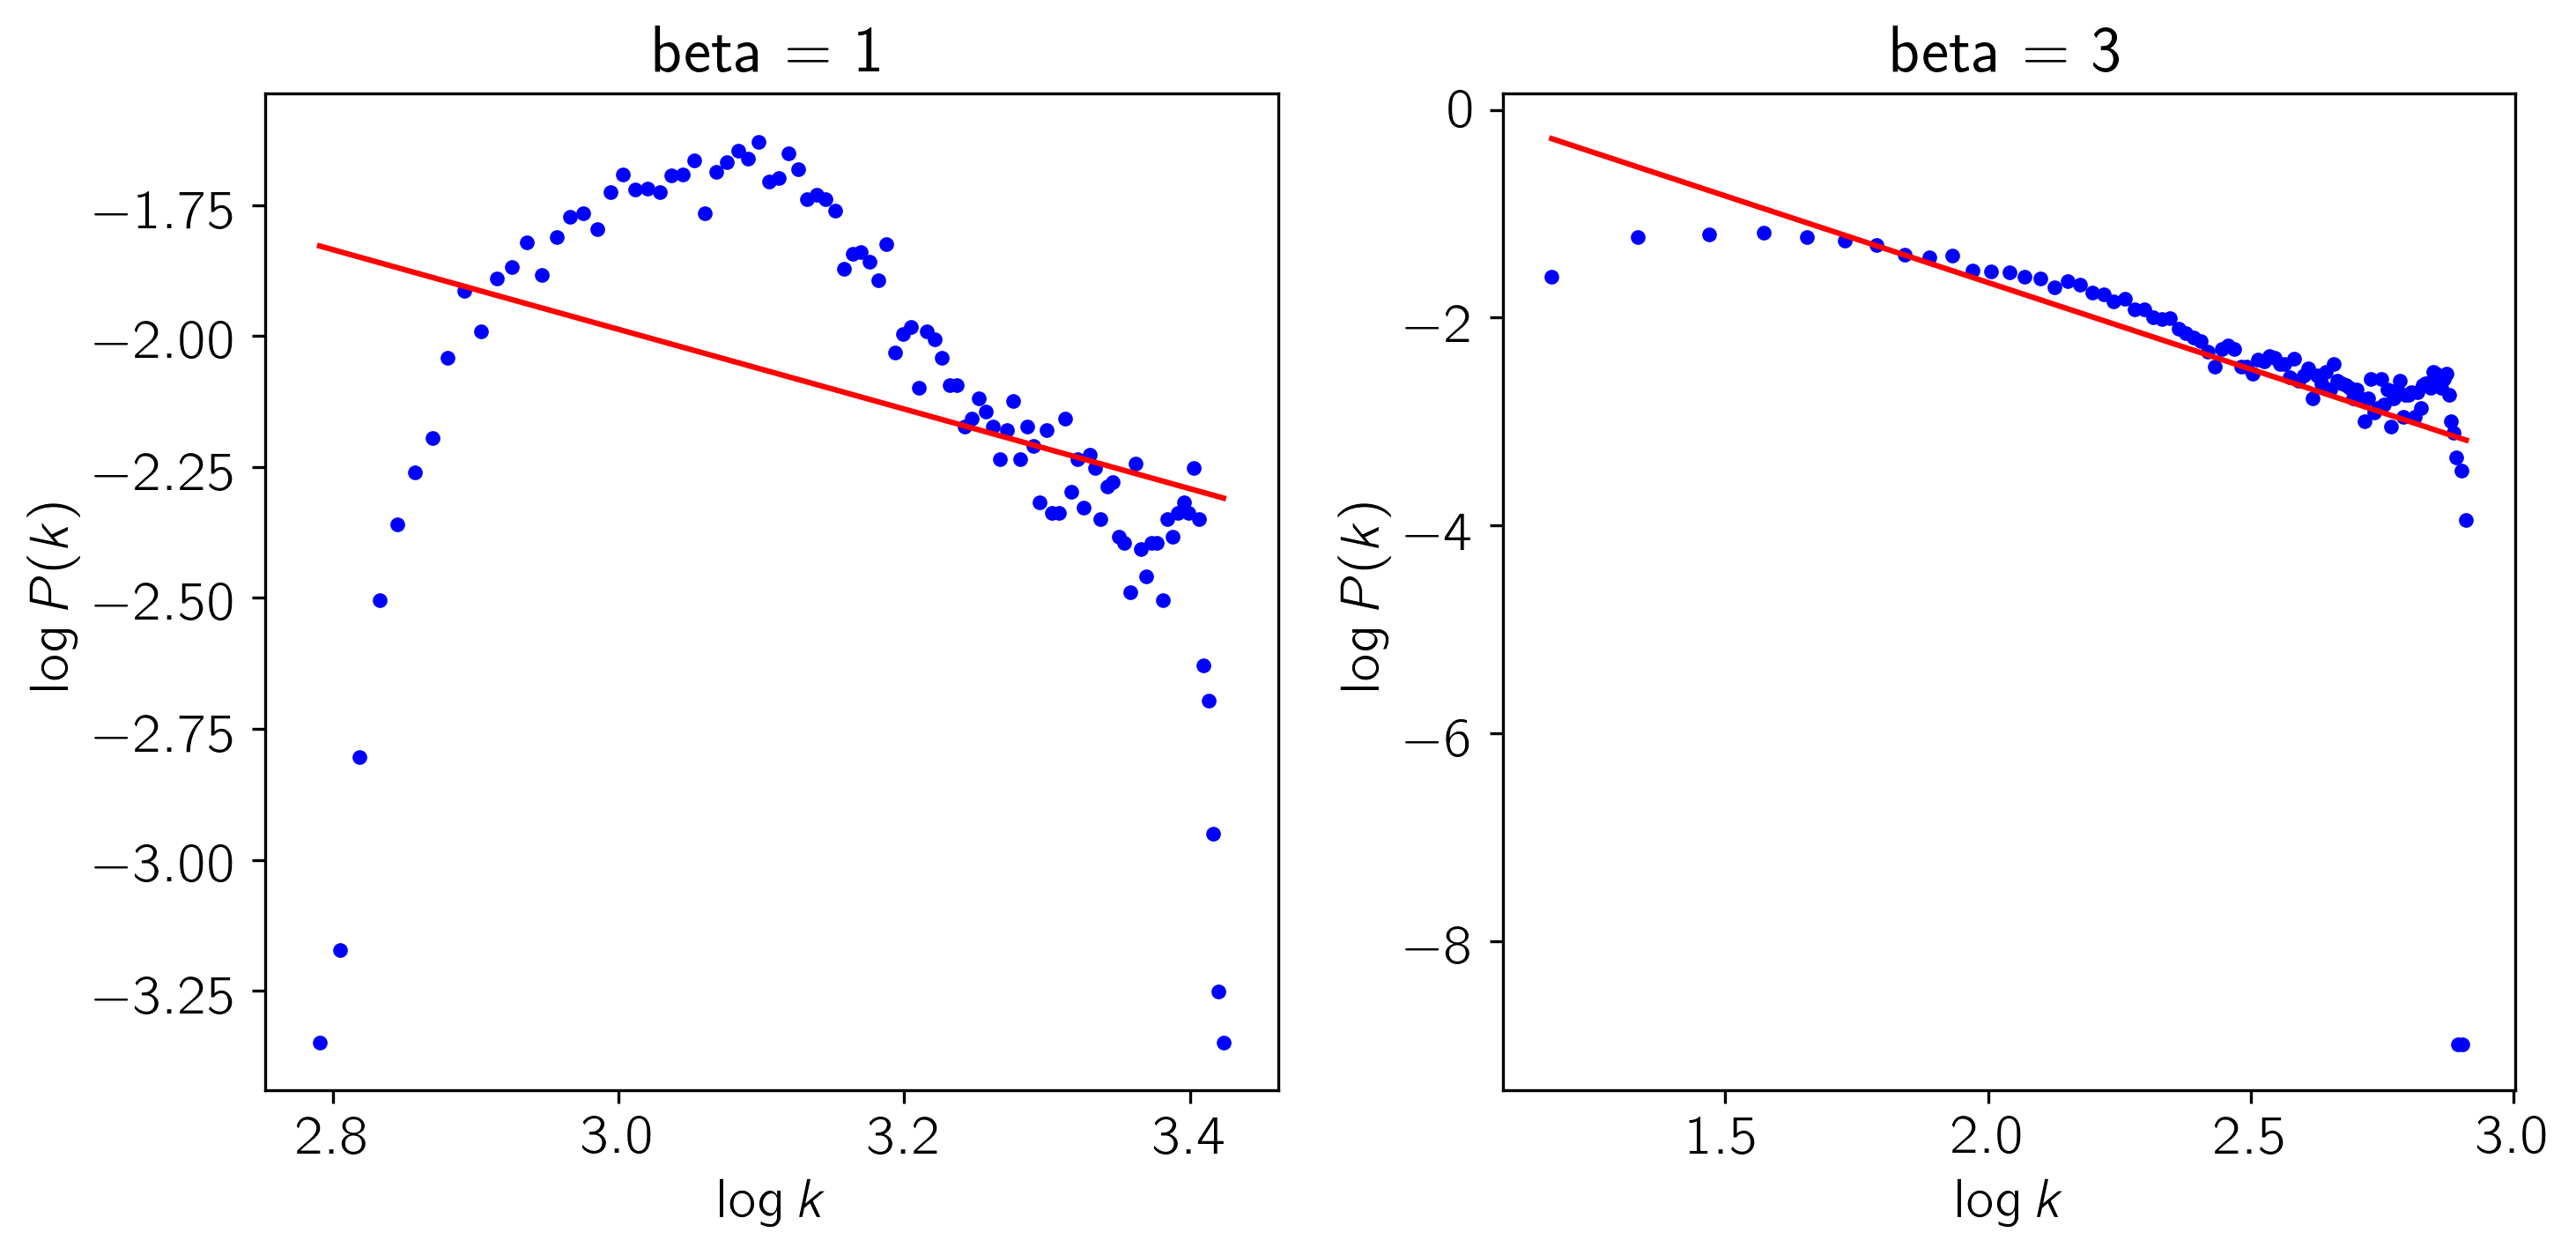
\includegraphics[clip,width=0.8\textwidth]{Figures/pick_beta.png}
  \caption{Degree distributions}
  \label{fig:beta}
\end{figure}

\subsection{Module detection}	
Once the network has been constructed, the next step is to study its structure and dynamics identifying communities also called modules. The idea is to cluster genes with similar expression change patterns. Membership in these modules may overlap in biological contexts, where modules may be related to specific molecular, cellular or tissue functions and the biological components (i.e. genes) are involved in multiple functions.\\

To identify these overlapping communities we make use of the Hierarchical Link Clustering (HLC) algorithm proposed in~\cite{ahn2010link}. HLC approach reinvent communities as groups of links rather than nodes, each node inherits all memberships of its links and can thus belong to multiple, overlapping communities. The algorithm maps links to nodes and connects them if a pair of links shares a node. They compute the similarity between links using the Jaccard index for unweighted networks and the Tanimoto coefficient for weighted networks. With this similarity, they use single-linkage hierarchical clustering to build a dendrogram where each leaf is a link from the original network and branches represent link communities. Finally, the most relevant communities are established at the maximal partition density, a function  based on link density inside communities.\\

The current network represented by the adjacency matrix $A$, corresponds to a complete and weighted network of $8928$ genes (nodes) and $39850128$ edges. For computational reasons, this network was transformed into an unweighted one $\hat{A}$, keeping only the connections above the cutoff value of $0.2$. The resulting unweighted network has a total of $5810$ nodes and $16875145$ edges. After applying the HLC algorithm, a total of $4131$ genes were distributed in $5143$ overlapping modules of $3$ or more genes. Figure~\ref{fig:overlap} shows a histogram of the overlapping percentage of these genes, measured as the proportion of modules to which each gene belongs.\\

%overlapping percentage
\begin{figure}[h]
  \centering
    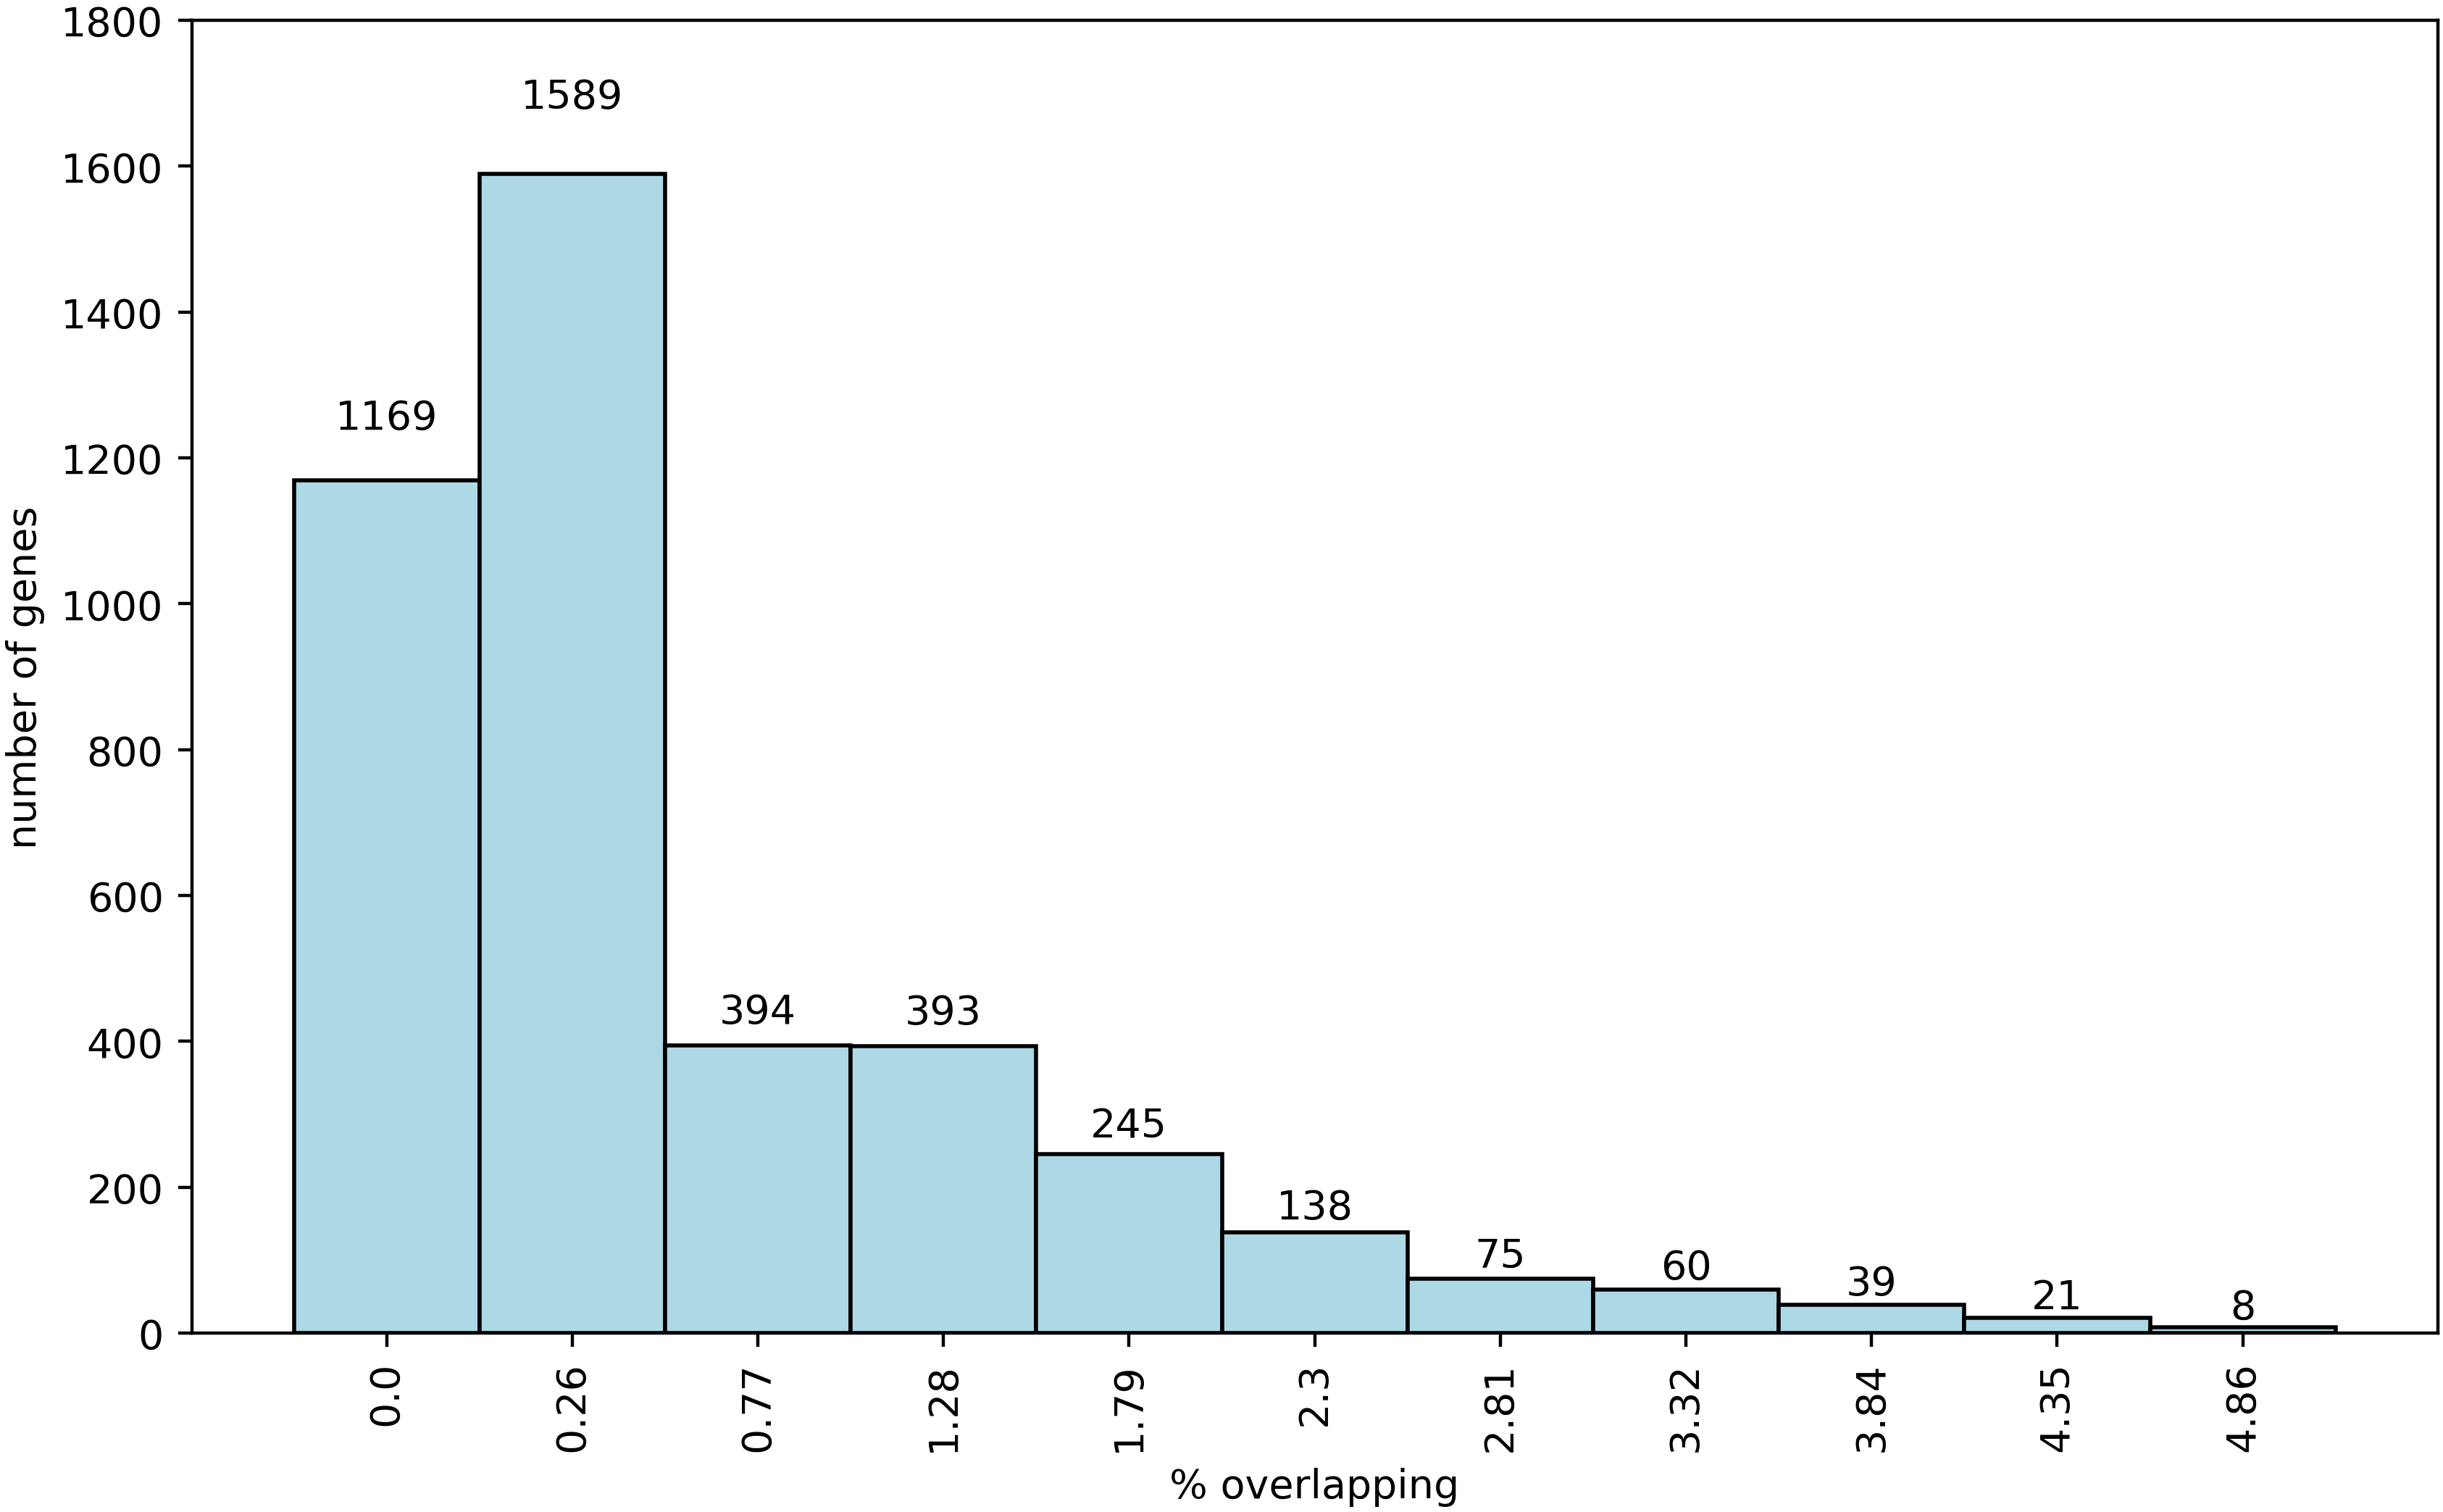
\includegraphics[clip,width=0.4\textwidth]{Figures/artificial_modules.png}
  \caption{Overlapping percentage}
  \label{fig:overlap}
\end{figure}

\subsection{Modules association to phenotypic traits}
Our approach to identify the most relevant gene groups (modules) in the response to salt stress, consists in relating the co-expression network with phenotypic data from the samples. We use 3 phenotypic traits: shoot $K^+$ content, root biomass and shoot biomass. These were measured for the 92 genotypes studied, under  control and salt stress conditions. These data can be found in the supplementary information of~\cite{campbell2017allelic}. As shown in Figure \ref{fig:pdata}, there are significant differences in the values of these phenotypic traits between both stress and control conditions. This supports the idea that these variables represent tolerance-associated traits in rice under salt stress.\\

% boxplots
\begin{figure}[h]
  \centering
    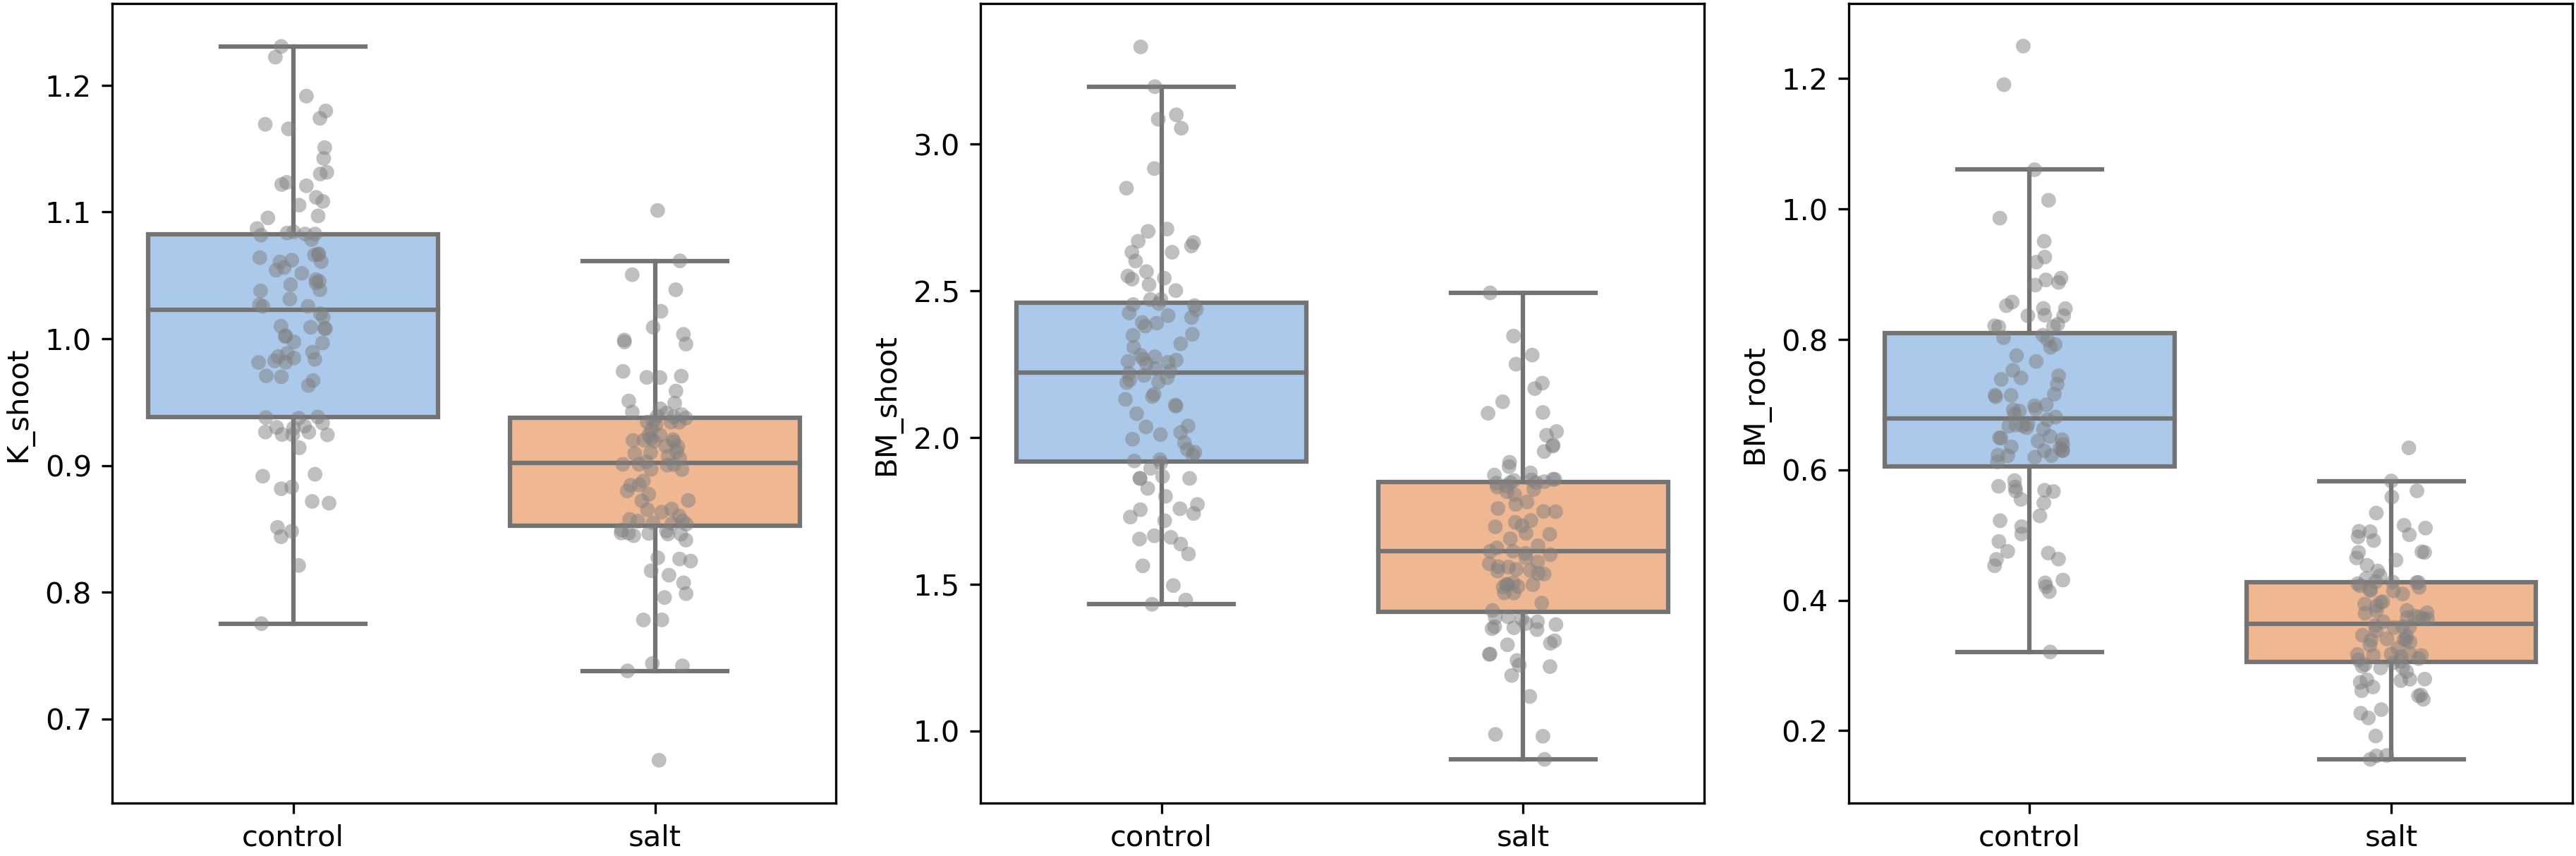
\includegraphics[clip,width=1\textwidth]{Figures/phenotypic_traits.png}
  \caption{Phenotipic traits distribution under control and salt stress}
  \label{fig:pdata}
\end{figure}

In order to relate the modules to the phenotypic traits, we represent each module with the first principal component of the Log Fold Change submatrix, corresponding to the genes of such module, which can be thought of as an average differential expression profile for each community. These profiles are then associated with each phenotypic trait using the LASSO variable selection method, allowing to identify a set of relevant modules related to the response to salinity conditions in rice plants. See Appendix A for a LASSO method description.\\

In our case study, 6 modules were detected as relevant in the response to salt stress in rice: 3 modules of 3 genes each one associated with shoot K content, 2 modules of 3 genes associated with  shoot biomass, and 1 module of 4 genes associated with root biomass.\\

\subsection{Genes enrichment}
% genes seleccionados con expresión diferencial según análisis DEA. 
% gene ontology de esos genes
% redes de interacción PP de los genes nombrados

\section{Discussion}


\bibliographystyle{acm}
\bibliography{mybibliography}

\newpage
\section*{Appendix}
\subsection{A: Variable selection with LASSO}
LASSO (Least Absolute Shrinkage Selector Operator) is a regularized linear regression technique, a method that combines a regression model with a procedure of contraction of some parameters towards zero and selection of variables, imposing a restriction or a penalty on the regression coefficients. Very useful in problems where the number of variables (genes) $ n $ is much greater than the number of samples $ p $ ($ n \gg p $). Lasso solves the least squares problem with restriction on the $ L_1$-norm of the coefficient vector:

\begin{equation}
\min \left\lbrace\sum_{i=1}^{p}{\left( y_i-\sum_{j=1}^n{\beta_j x_{ij}}\right)^2} \right\rbrace , \textrm{sujeto a} \sum_{j=1}^n\abs{\beta_j}\leq s
\end{equation}

Or equivalently minimizing:
\begin{equation}
\sum_{i=1}^{p}{\left( y_i-\sum_{j=1}^n{\beta_j x_{ij}}\right)^2} + \lambda \sum_{j=1}^n\abs{\beta_j}
\end{equation}
being $ s $, $ \lambda \geq 0 $ the respective penalty parameters for complexity.\\

%LASSO produces parameter estimation and simultaneous variable selection for increasing values of $ \lambda $.

%if $ \lambda = 0 $ the estimator corresponds to the ordinary least squares estimator.

Since the $\lambda$ value determines the degree of penalty, the accuracy of the model depends on its choice. Cross-validation is often used to select the regularization parameter, choosing the one that minimizes the mean-squared error. With that selected $\lambda$ value, the model is adjusted again, this time using all the observations.\\

In the module gene selection context, the outcome variable correspond to the phenotypic trait, whereas the predictors are the modules, detected by the hierarchical clustering, represented by the first principal component of the module. After running the Lasso regression will select the most significant modules associated with phenotypic data.  


\end{document}
